\documentclass[border=5pt]{standalone}
\usepackage{tikz}
\usepackage{xcolor}
\usetikzlibrary{positioning,shapes.geometric,arrows.meta,fit,backgrounds,calc}

\definecolor{stage1}{RGB}{66,133,244}
\definecolor{stage2}{RGB}{52,168,83}
\definecolor{stage3}{RGB}{251,188,5}
\definecolor{stage4}{RGB}{234,67,53}

\begin{document}
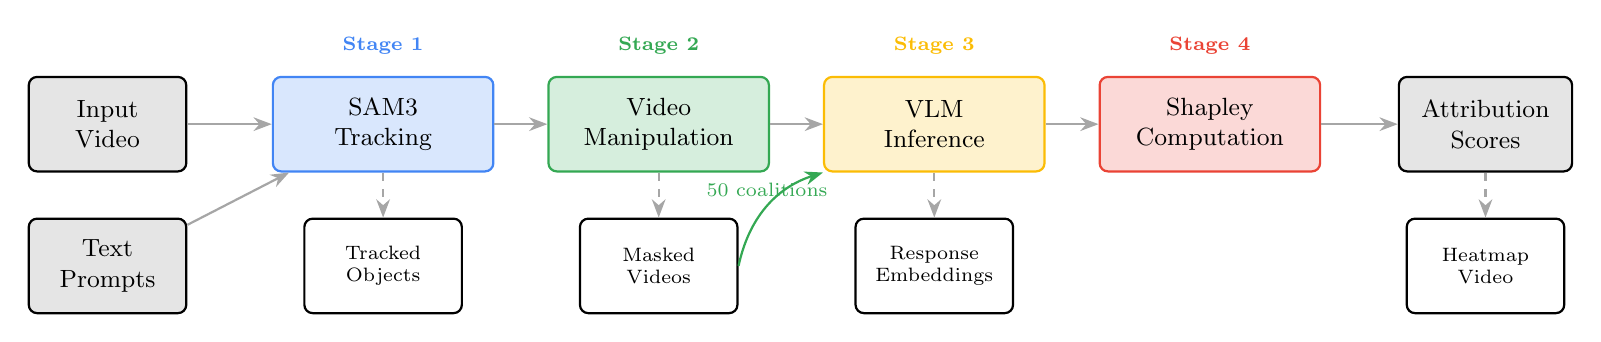
\begin{tikzpicture}[
    box/.style={draw, thick, rounded corners=3pt, minimum height=1.2cm, align=center, font=\small},
    stage/.style={box, minimum width=2.8cm},
    arrow/.style={-{Stealth[scale=1.0]}, thick, gray!70},
    label/.style={font=\scriptsize\bfseries}
]

% Input
\node[box, fill=gray!20, minimum width=2cm] (input) at (0,0) {Input\\Video};
\node[box, fill=gray!20, minimum width=2cm] (prompts) at (0,-1.8) {Text\\Prompts};

% Stage 1: Tracking
\node[stage, fill=stage1!20, draw=stage1] (track) at (3.5,0) {SAM3\\Tracking};
\node[label, stage1] at (3.5, 1) {Stage 1};

% Stage 2: Manipulation
\node[stage, fill=stage2!20, draw=stage2] (manip) at (7,0) {Video\\Manipulation};
\node[label, stage2] at (7, 1) {Stage 2};

% Stage 3: VLM
\node[stage, fill=stage3!20, draw=stage3] (vlm) at (10.5,0) {VLM\\Inference};
\node[label, stage3] at (10.5, 1) {Stage 3};

% Stage 4: Shapley
\node[stage, fill=stage4!20, draw=stage4] (shapley) at (14,0) {Shapley\\Computation};
\node[label, stage4] at (14, 1) {Stage 4};

% Output
\node[box, fill=gray!20, minimum width=2.2cm] (output) at (17.5,0) {Attribution\\Scores};

% Intermediate outputs (below)
\node[box, fill=white, minimum width=2cm, font=\scriptsize] (tracks) at (3.5,-1.8) {Tracked\\Objects};
\node[box, fill=white, minimum width=2cm, font=\scriptsize] (masked) at (7,-1.8) {Masked\\Videos};
\node[box, fill=white, minimum width=2cm, font=\scriptsize] (responses) at (10.5,-1.8) {Response\\Embeddings};
\node[box, fill=white, minimum width=2cm, font=\scriptsize] (viz) at (17.5,-1.8) {Heatmap\\Video};

% Arrows
\draw[arrow] (input) -- (track);
\draw[arrow] (prompts) -- (track);
\draw[arrow] (track) -- (manip);
\draw[arrow] (manip) -- (vlm);
\draw[arrow] (vlm) -- (shapley);
\draw[arrow] (shapley) -- (output);

\draw[arrow, dashed] (track) -- (tracks);
\draw[arrow, dashed] (manip) -- (masked);
\draw[arrow, dashed] (vlm) -- (responses);
\draw[arrow, dashed] (output) -- (viz);

% Coalition loop
\draw[arrow, stage2, thick] (masked.east) to[bend left=30] node[above, font=\scriptsize] {50 coalitions} (vlm.south west);

\end{tikzpicture}
\end{document}
